\phantomsection
%\addcontentsline{toc}{chapter}{Introduzione}
\chapter{Introduzione}
\markboth{Introduzione}{}
% [titolo ridotto se non ci dovesse stare] {titolo completo}

\section{Motivazioni e Obiettivi} %\label{1sec:scopo}
L'evoluzione da dati tradizionali a dati complessi (e.g., multimediali, geografici e fuzzy) e successivamente ai big data, ha sollevato la necessit\`{a} di progettare metodi e strumenti per estrarre automaticamente e visualizzare le informazioni e statistiche da questi. Queste statistiche includono le classificazioni, le regole di associazione e diversi tipi di metadata \cite{profiling-relational-data}, come i value patterns, le foreign keys e le dipendenze dei dati, del tipo multivalore, inclusione e \acrlong{fds} (\acrshort{fds}) \cite{surveydatabasedependency}. Queste ultime venivano usate principalmente nei tradizionali database alfanumerici a scopi di normalizzazione\footnote{La \textbf{normalizzazione} \`{e} un processo atto ad eliminare le ridondanze ed il rischio di incoerenza dal database.}. Successivamente, con l'evoluzione delle tecnologie alla base dei database, nuovi tipi di \acrlong{fds} sono state definite, come ad esempio le Dipendenze Funzionali Fuzzy \cite{ffdandlljoin} e le Dipendenze Multimediali \cite{nomalizationframework}, le quali introducono alcune approssimazioni necessarie per confrontare dati complessi, ma anche per tener conto dei confronti testuali, dei valori mancanti, delle dipendenze parzialmente valide ed altre approssimazioni nel contesto di applicazioni per big data. A tal fine, sono state introdotte oltre trenta definizioni differenti di Dipendenze Approssimate, chiamate anche \acrlong{rfds} (\acrshort{rfds}) \cite{rfdsurvey}. Nel contesto dei big data, le \acrlong{rfds} insieme ad altri metadati di profilazione sono utilizzate per diversi scopi, tra cui pulizia dei dati, ottimizzazione delle query e cos\`{i} via. Tuttavia, in questo contesto potrebbe essere difficile specificare le \acrlong{rfds} in fase di progettazione, insieme ai parametri che definiscono il loro livello di approssimazione, come ad esempio la similitudine tra valori di attributi e le soglie per indicare la porzione di dataset su cui una \acrlong{rfd} risiede. Quindi, \`{e} stato necessario escogitare metodi per la ricerca automatica delle \acrlong{rfds} nei dati \cite{ddiscoveryfromdata}. La ricerca delle \acrlong{rfds} nei dati \`{e} possibile grazie alla disponibilit\`{a} di raccolte di big data, poich\'{e} forniscono un'elevata rilevanza statistica per dipendenze approssimative che altrimenti dovrebbero essere specificate in fase di progettazione, in base alla semantica dei dati. D'altro canto, sorgono due problemi principali con gli algoritmi di scoperta di \acrlong{rfds} applicati ai big data:
\begin{enumerate}
    \item complessit\`{a} computazionale,
    \item visualizzazione dei risultati.
\end{enumerate}
Il primo \`{e} un problema gi\`{a} sufficientemente complesso anche con le \acrlong{fds} tradizionali e la sua complessit\`{a} cresce considerabilmente con l'introduzione delle approssimazioni, specialmente quando il numero di attributi cresce. Il secondo problema riguarda la complessit\`{a} dei risultati, perch\'{e} gli algortimi di ricerca delle \acrlong{rfds} spesso restituiscono in output un enorme set di dipendenze, con molte combinazioni di soglie differenti, il che rende difficile per un utente ricavare informazioni utili da queste. Ad oggi non \`{e} stato fornito alcun metodo di visualizzazione per le \acrlong{rfds}. L'obiettivo, quindi, \`{e} quello di progettare uno strumento che faciliti l'individuazione e la lettura delle informazioni utili riguardanti le \acrlong{rfds}. La tecnica di visualizzazione da utilizzare si applica alle \acrlong{rfds} scoperte da dati multimediali e big data e rappresenta sia le dipendenze scovate sia le loro soglie, includendo una strategia di classificazione che mira a selezionare le \acrlong{rfds} pi\`{u} rilevanti e significative su un determinato dataset.

\section{Risultati}
\begin{figure}[ht]
    \centering
    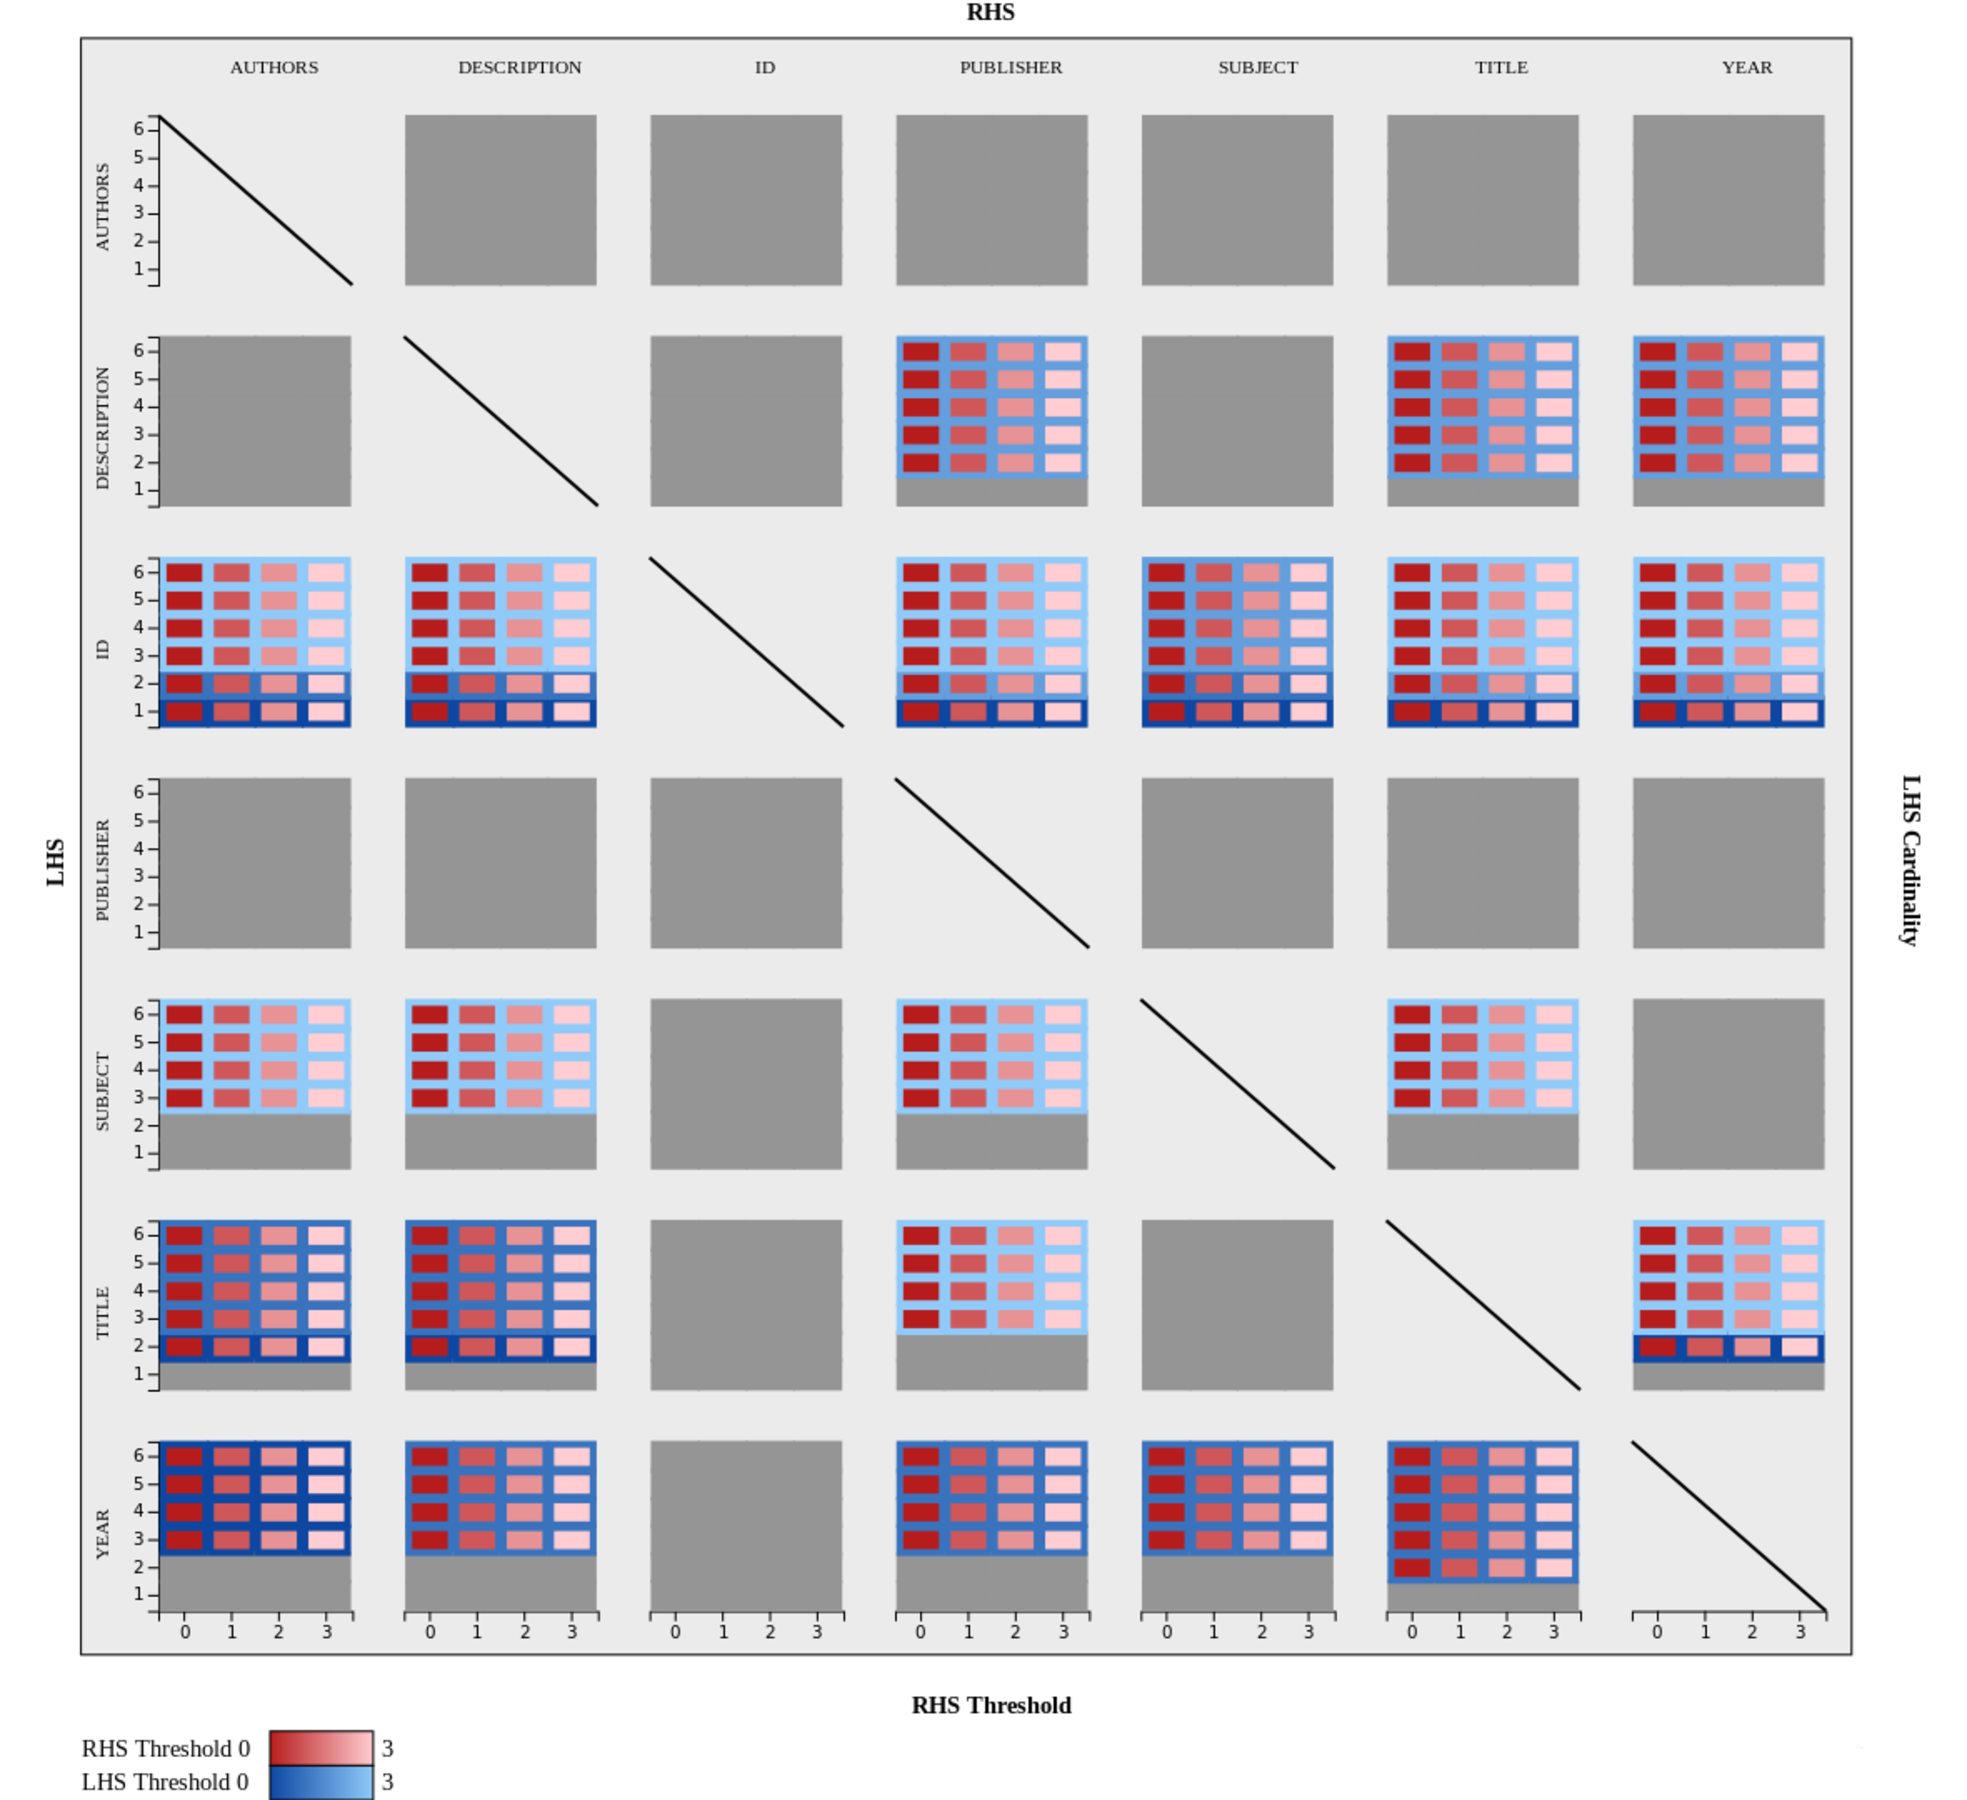
\includegraphics[width=\linewidth]{capitoli/figure/citiseer_2000_result}
    \caption{Rappresentazione ottenuta in output da Dependensee del dataset Citiseer 2000.}
    \label{fig:citiseer_2000_result}
\end{figure}
\begin{figure}[ht]
    \centering
    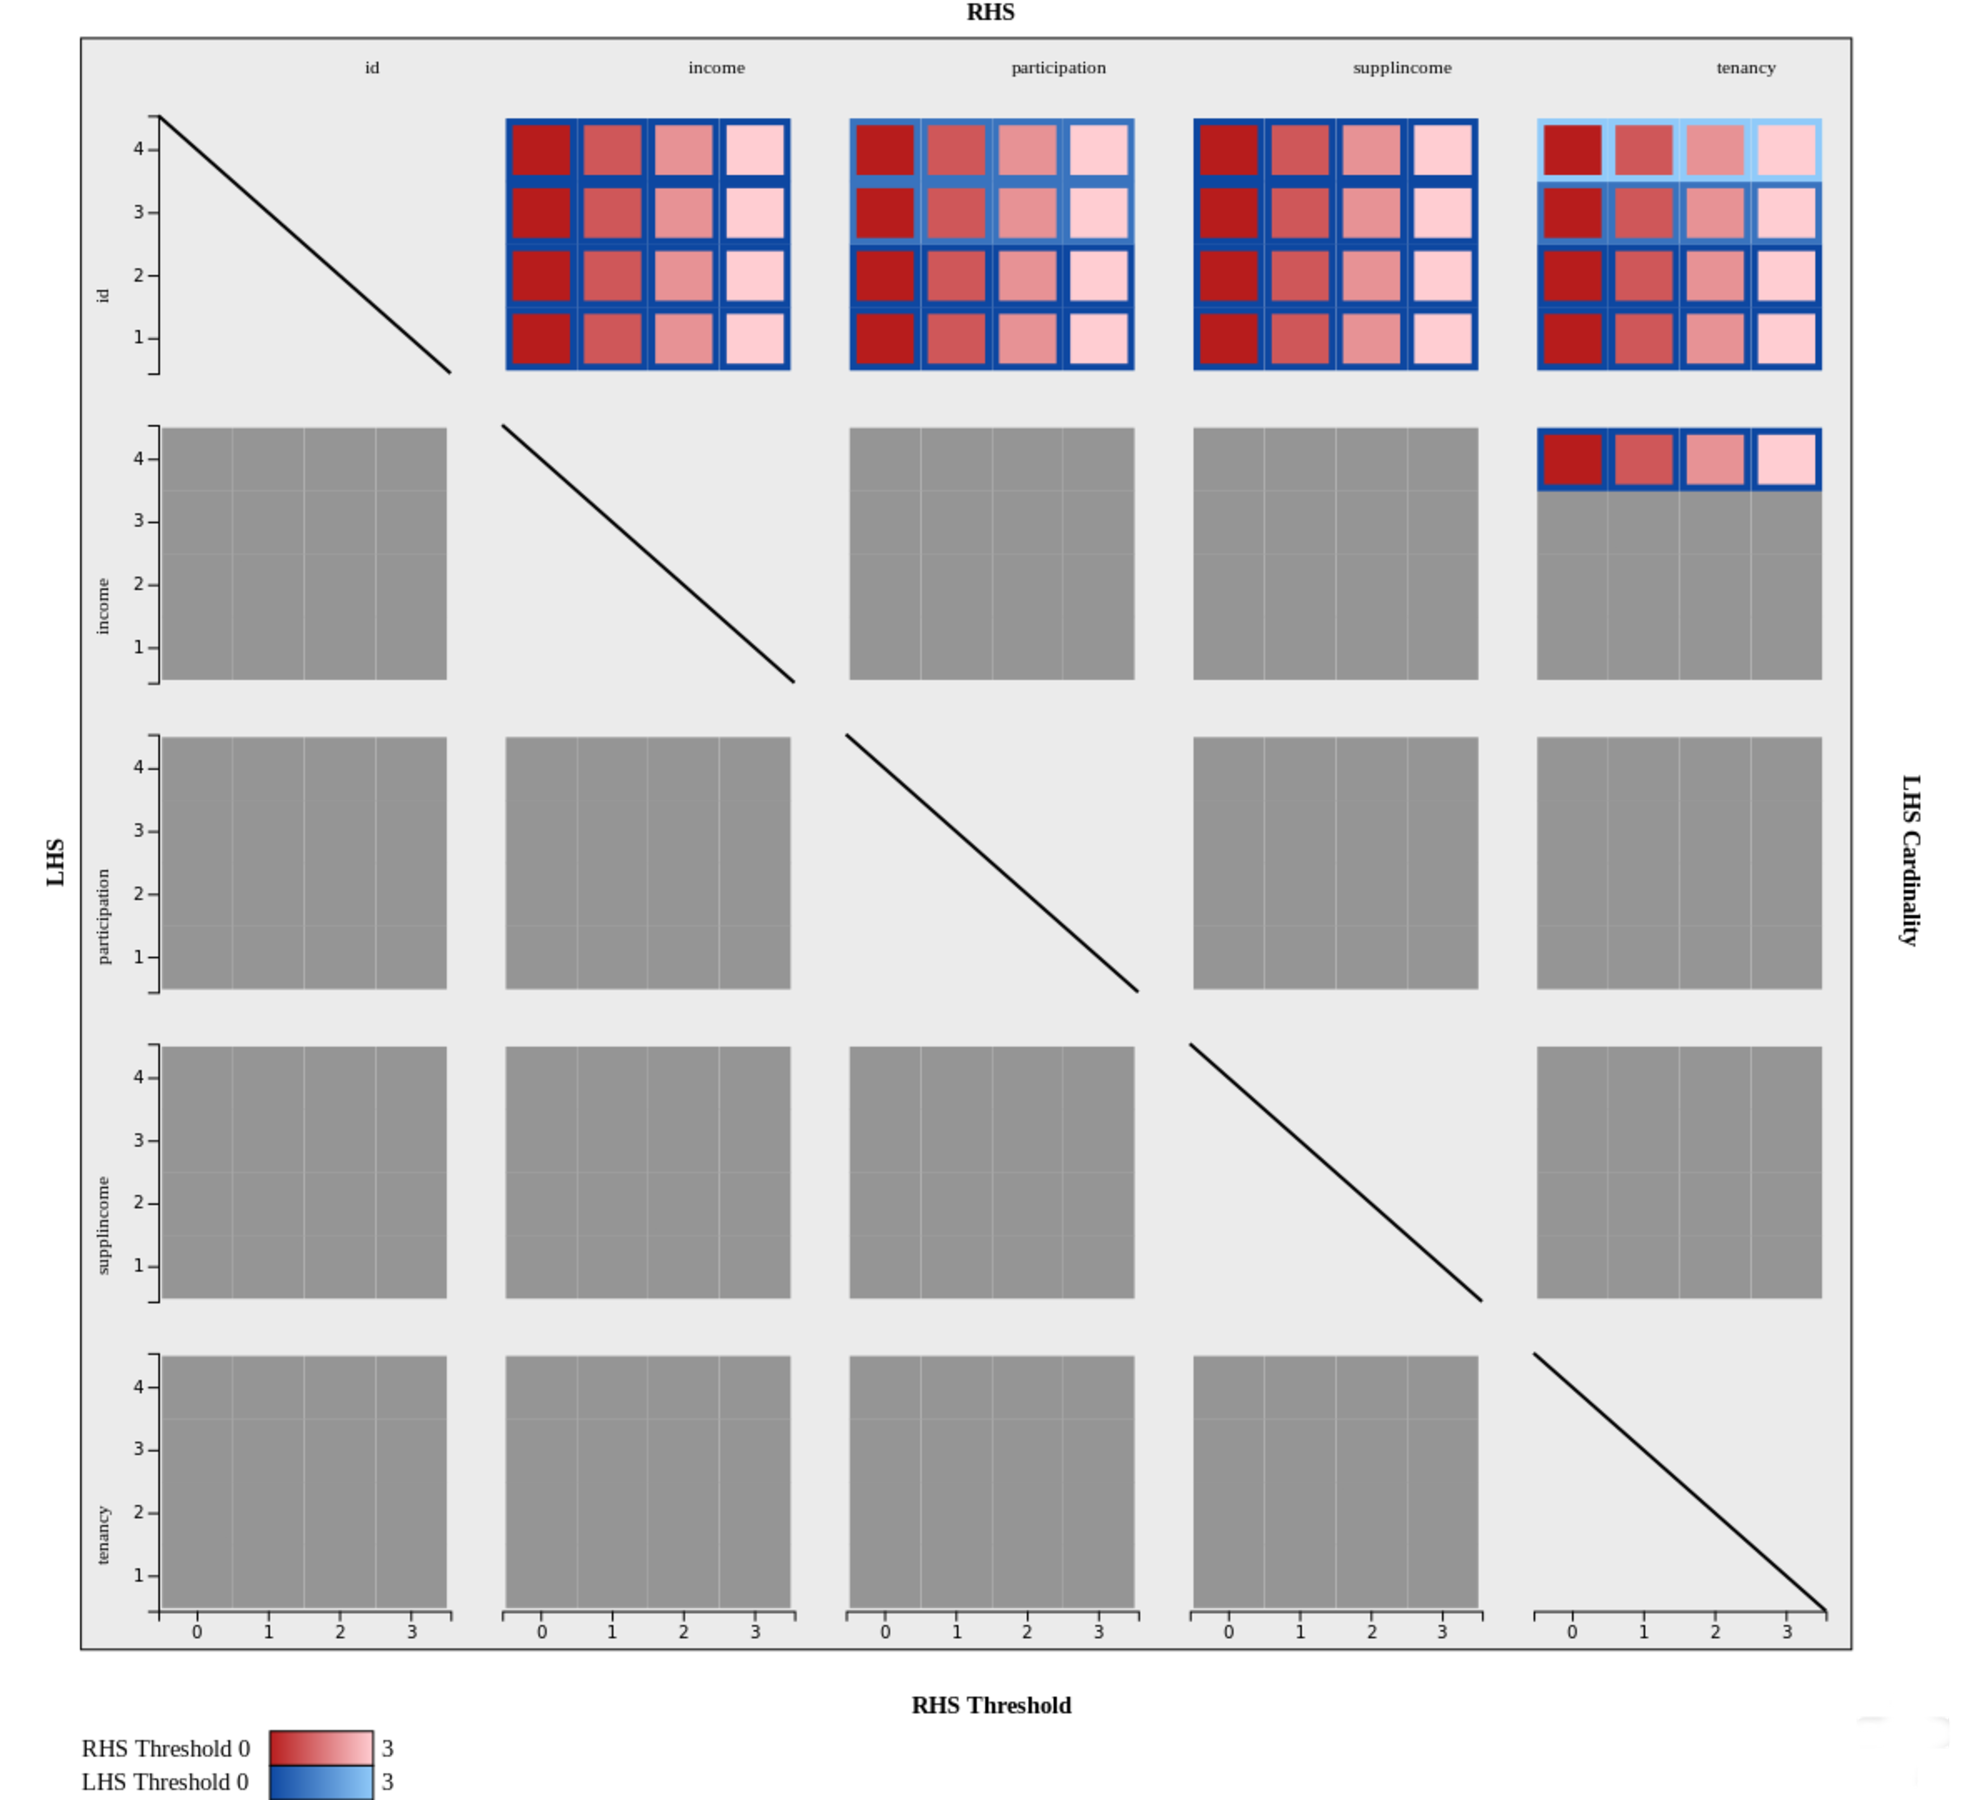
\includegraphics[width=\linewidth]{capitoli/figure/foodstamp_result}
    \caption{Rappresentazione ottenuta in output da Dependensee del dataset Foodstamp.}
    \label{fig:foodstamp_result}
\end{figure}
Attraverso l'implementazione della metafora di visualizzazione esposta nel capitolo \ref{section:visual_rep_metaphore} all'interno di Dependensee, esposto nel capitolo \ref{cap5:dependensee}, si \`{e} riusciti a rappresentare in modo immediato ed efficace un dataset di \acrlong{rfds}. In questo modo \`{e} stato possibile effettuare un'analisi visiva quasi istantanea, grazie alle diverse caratteristiche messe in luce dalla rappresentazione grafica fornita dallo strumento. Infatti, questa rappresentazione raffigura le dipendenze minimali esistenti tra tutti gli attributi contenute nel dataset, mettendo in risalto la cardinalit\`{a} del lato sinistro e le thresholds associate sia per il lato sinistro che per il lato destro.\par
La Figura \ref{fig:citiseer_2000_result} mostra la rappresentazione grafica ottenuta analizzando il dataset \textit{Citiseer 2000} con il tool proposto. Da un primo sguardo si pu\`{o} notare come questa faciliti effettivamente l'analisi visiva per l'utente. Analizzando il dataset attraverso tale rappresentazione possiamo notare, mediante la diagonale nulla, come le \acrlong{rfds} banali non vengano rappresentate. Se prendiamo in considerazione la prima riga, possiamo notare come non esistano \acrlong{rfds} minimali con l'attributo \texttt{AUTHORS} sul lato sinistro e con almeno un attributo diverso sul lato destro. Mentre, con la colonna relativa all'attributo \texttt{ID}, possiamo notare l'assenza di \acrlong{rfds} minimali con l'attributo relativo sul lato destro. Se analizziamo la sotto-matrice relativa all'attributo riga \texttt{TITLE} ed all'attributo colonna \texttt{AUTHORS}, possiamo notare l'assenza di \acrlong{rfds} con cardinalit\`{a} pari a 1 e l'esistenza di \acrlong{rfds} minimali con threshold pari a 0 sul lato sinistro e cardinalit\`{a} pari a 2, mentre per cardinalit\`{a} maggiori vi sono \acrlong{rfds} con threshold diverse da 0 ma con valori vicini a questo.\par
Consideriamo adesso il dataset \textit{Foodstamp}. La Figura \ref{fig:foodstamp_result} mostra la rappresentazione grafica ottenuta dando in input il dataset a Dependensee, il tool proposto. Dal grafico ottenuto possiamo notare, attraverso la prima riga, come le uniche dipendenze esistenti siano con l'attributo \texttt{id} sul lato sinistro e, attraverso la seconda riga, con l'attributo \texttt{income} sul lato sinistro. Le prime sono in relazione con tutti gli altri attributi del dataset, infatti le colonne relative alla prima riga sono tutte colorate. Mentre, per l'attributo \texttt{income}, possiamo notare l'esistenza di \acrlong{rfds} solo con l'attributo \texttt{tenancy} sul lato destro. Con le righe e le colonne restanti possiamo notare che non vi sono \acrlong{rfds}, difatti sono colorate in grigio.

\section{Struttura della tesi}
La tesi \`{e} strutturata come segue. Il capitolo \ref{cap2:stato_arte} esamina gli approcci esistenti in letteratura per visualizzare i metadati estratti dai big data. Il capitolo \ref{cap3:fd} fornisce alcune definizioni di background sulle \acrlong{rfds} ed una breve introduzione sugli algoritmi per la loro estrazione dai dati. Il capitolo \ref{cap4:visual_representation} introduce il concetto di minimalit\`{a} per filtrare le \acrlong{rfds} rilevanti ed una metafora di visualizzazione per rappresentare tali dipendenze. Il capitolo \ref{cap5:dependensee} introduce \textit{Dependensee}, il tool sviluppato durante il lavoro di tesi per la visualizzazione di insiemi minimali di \acrlong{rfds}.